%! TEX root = 'main.tex'

\section{Evaluation}
\label{sec:ktoctou-evaluation}

In this section, we evaluate \name's performance overhead and how it protects the operating system from real-world vulnerabilities.


\subsection{Performance}
In this section, we focus on performance evaluation.
As previously mentioned, \name has two key components, the system module and the hypervisor. To present the performance impact introduced by this mitigation, we conduct the tests in three parts. 

All tests run on the PC with Intel Core I5-6400 (6 GEN CPU Skylake), ASUS H110M-C motherboard (Intel H110 Chipset, Realtek RTL8111H Network Controller), 8GB RAM, and 500GB hard disk.

\textbf{textit{Benchmarks.}} The hypervisor plays an essential part in \name. Without the hypervisor confining the SMAP feature, it would not be possible to debug a complex system like Windows with a system-wide unsupported feature. Nowadays, a hypervisor is part of the cloud computing infrastructure and can be regarded as a built-in component. The Windows 10 operating system even brings its native hypervisor to deliver security goals. Under those circumstances, \name can be added to the existing hypervisor with less performance overhead imposed on the system. 

To evaluate the hypervisor's performance overhead, we use the well-known benchmark SPEC 2006. We understand that this benchmark is for processor instruction evaluation, specifically for microarchitectural aspects, such as instruction execution, branch prediction accuracy, cache policies. We choose several programs from the set. They are all non-GUI and computational intensive programs. Therefore the performance overhead incurred is primarily due to the hypervisor. Although our hypervisor and Windows HVCI have different objectives, we compare them to show that run-time protection utilizes virtualization techniques is practical.

\begin{figure}[th]
  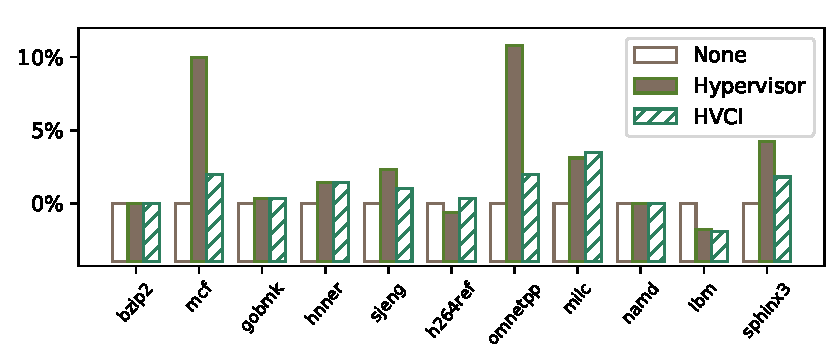
\includegraphics[width=0.47\textwidth]{figures/benchmark3}
  \centering
  \caption{Performance overhead on the SPEC benchmarks incurred by the run-time load hypervisor. HVCI represent the Windows 10 native hypervisor for Hypervisor-Protected Code Integrity. All overheads are normalized to the unprotected system running benchmark.}
  \label{fig:ktoctou-benchmark}
\end{figure}


\autoref{fig:ktoctou-benchmark} shows that hypervisor's performance overhead is acceptable, on average, 3.25\%. HVCI yields a modest performance overhead of 0.81\%.

% show my respect.. maybe remove it later

Our hypervisor is slower than HVCI, particularly in two benchmark programs. Learning more about computer architecture and virtualization techniques, we wish to improve our hypervisor to perform better.



\textbf{\textit{Non-trivial Applications.}} We also evaluate \name on several non-trivial applications, as shown in~\autoref{fig:ktoctou-performance}. The applications we choose are meaningful because the kernel-TOCTOU vulnerability may threaten them. For example, a web server such as Nginx normally runs in a non-root account and takes external requests. 

To test web servers, we count their response time for a web request. For compression software, the test is to compress large files. We also use speedtest1.c, which is a performance testing program for sqlite3. The result shows that the performance overhead is acceptable. 

\begin{figure}[th]
  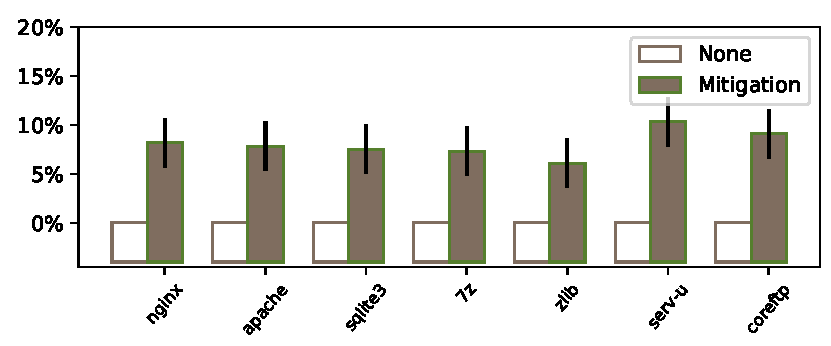
\includegraphics[width=0.47\textwidth]{figures/performance4}
  \centering
  \caption{Performance overhead in non-trivial applications. Overhead mostly being introduced on system calls that need to fetch user parameters}
  \label{fig:ktoctou-performance}
\end{figure}





\textbf{\textit{GUI.}} Through our investigation, we find that the Windows graphical subsystem, namely, Win32k.sys, has the most double-fetch issues.  Because GUI programs need to redraw their graphical components frequently, they invoke the win32k system calls a lot, even for a simple program such as Windows notepad. Therefore,  our mitigation incurs an unneglectable performance over GUI programs. The overhead is primarily affected by how often the interface is refreshed. For example, if minimizing a GUI program's window, its performance will not be slow down by the graphical interface at all. We compare GUI programs with non-GUI programs in the following aspects: the number of user pages accessed by kernel per system call and how many double fetches occur. We drag the GUI program's window to trigger redraw, and we send one URL request to the web servers per second. The measurement takes the first 500 system calls.

\begin{center}
\begin{table}[ht]
	\small
	%\renewcommand{\arraystretch}{1.3}
	\caption{System call count and user-pages accessed for GUI \& non-GUI programs }
	\label{table:pages}
	\centering
%	\begin{tabular}{ l|p{0.04\textwidth}|p{0.108\textwidth}|l|p{0.045\textwidth}|p{0.045\textwidth} } 
%	\begin{tabular}{ c@{}|@{}c@{}|@{}c@{}|@{}c@{}|@{}c@{}|@{}c }   
	\begin{tabular}{@{}>{\centering\arraybackslash}m{1.40cm}@{}|
			@{}>{\centering\arraybackslash}m{1.15cm}@{}|
			@{}>{\centering\arraybackslash}m{2.30cm}@{}|
			c|
			@{}>{\centering\arraybackslash}m{1.15cm}@{}|
			@{}>{\centering\arraybackslash}m{0.97cm}@{} } 
		\hline
		Programs & System Calls & Protected Pages(r, w) & \textbf{avg.} & Double Fetch & Time (ms)\\ 
		\hline
		nginx & 500 & 711(711, \textbf{0}) & 1.42 & \textbf{223} &12312\\ 
		apache & 500 & 689(689, \textbf{0})  & 1.38 & \textbf{205} &11339\\ 
		notepad & 500 & 1434(1102, 241) & 2.87 & \textbf{1373} & 1859 \\ 
		freecell & 500 & 1352(1165, 187) & 2.70 & \textbf{1266} & 1500 \\ 
		\hline
	\end{tabular}
\end{table}
\end{center}


\autoref{table:pages} shows some interesting results. Refreshing the GUI takes tremendous system calls. As expected, both the kernel and the Win32k subsystem accesses user pages, but the win32k accesses more than the kernel. They both \textit{capture} the user parameters at each system call, but the win32k module read/write more user data even in the middle of a system call.


We also count the number of reads and writes on user pages. For non-GUI programs, the number of writes is zero, which is strange because most system calls need to write results back to the user program. With investigation, the causes are as follows. Windows provides three methods to transfer data between system calls and user programs, namely, Buffered I/O, Direct I/O, and Neither Buffered Nor Direct I/O. Among the three, the kernel mostly uses Buffer I/O and Direct I/O, which do not need to write to user-mode buffer directly. However, the kernel still needs to write user-mode variable such as the filehandle in system call \texttt{NtCreateFile}.
~\autoref{fig:probecode} shows the pseudo-code similar to what the kernel uses to validate user parameters. We can see that the code always reads the variable first and the SMAP exception only captures first access. Therefore, this coding style is another cause for the zero writes. The results show the kernel is well regulated on accessing user data. On the other side, the Win32k module has many writes, which tell a different story.


\begin{figure}[th]
  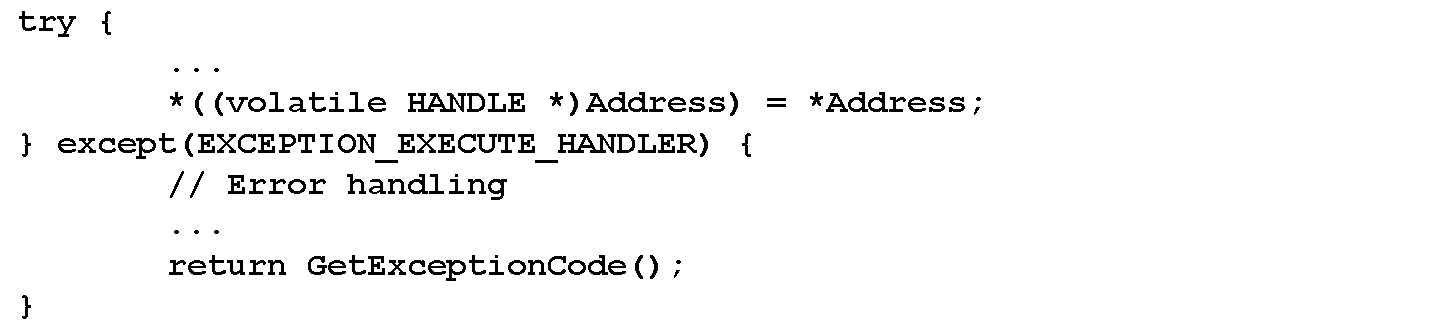
\includegraphics[width=0.47\textwidth]{figures/probecode}
  \centering
  \caption{Pseudo-code for validating a file handler.}
  \label{fig:probecode}
\end{figure}



% for later reference
%Buffered I/O
%The operating system creates a nonpaged system buffer, equal in size to the application's buffer. The I/O manager copies user data into the system buffer for write operations before calling the driver stack. For read operations, the I/O manager copies data from the system buffer into the application's buffer after the driver stack completes the requested operation.
%
%Direct I/O
%The operating system locks the application's buffer in memory. It then creates a memory descriptor list (MDL) that identifies the locked memory pages and passes the MDL to the driver stack. Drivers access the locked pages through the MDL.
%
%Neither Buffered Nor Direct I/O
%The operating system passes the application buffer's virtual starting address and size to the driver stack. The buffer is only accessible from drivers that execute in the application's thread context.
%




The column \textit{Double Fetch} shows the user-addresses that are read more than once during individual system calls. We trace this information with the fuzzing tool as previously introduced in~\autoref{sec:ktoctou-experiment}. Many of those double-fetch records are duplicates and benign. The kernel needs to read data from Process Environment Block (PEB) or Thread Environment Block (TEB), data structures located in userspace.  However, the Win32k module has many more cases. ~\autoref{table:doubleread} gives a glimpse of them. Every two rows indicate a double-fetch case, where after the first read, the subsequent instruction revisits the same address shortly after, and the identical CR3 and TEB show that two fetches are from the same thread of the same process.

Furthermore, with reverse-engineering effort, we find that in some of those cases, the Win32k module directly read the user variable and without the protection of a try-catch block. It is dangerous. The user programs can free the user memory and cause the kernel code to access an invalid page without protection, which leads to a crash.


\begin{center}
	\begin{table}[ht]
		\small
		%\renewcommand{\arraystretch}{1.2}
		\caption{In the selected double-fetch results, for every two lines, they have the same CR3 and TEB, which indicate the two records are from the same process, same thread. The two EIP are shortly apart, but the addresses they reference are the same and from userspace.}
		\label{table:doubleread}
		\centering
		%\begin{tabular}{ l l l l }
		\begin{tabular}{@{}>{\centering\arraybackslash}m{2.05cm}@{}|
				@{}>{\centering\arraybackslash}m{2.05cm}@{}|
				@{}>{\centering\arraybackslash}m{2.05cm}@{}|
				@{}>{\centering\arraybackslash}m{2.05cm}@{} } 
			\hline
			Cr3 & Eip & Addr. & Teb \\
			\hline
			0x6d40320 & 0xbf812de4 & \textbf{0x4808c4} & 0x7ffdd000 \\
			0x6d40320 & 0xbf812e4b & \textbf{0x4808c4} & 0x7ffdd000 \\
			\hline
			0x6d40320 & 0xbf812dea & \textbf{0x4808c8} & 0x7ffdd000 \\
			0x6d40320 & 0xbf812e55 & \textbf{0x4808c8} & 0x7ffdd000 \\
			\hline
			0x6d40320 & 0xbf812daf & \textbf{0x480750} & 0x7ffdd000 \\
			0x6d40320 & 0xbf812e21 & \textbf{0x480750} & 0x7ffdd000 \\
			\hline
			0x6d40320 & 0xbf80c04d & 0x7ffdd206 & 0x7ffdd000 \\
			0x6d40320 & 0xbf812ebe & 0x7ffdd206 & 0x7ffdd000 \\
			\hline
		\end{tabular}
	\end{table}
\end{center}



%Part of the overhead is introduced due to the overall intercepting of page fault exceptions of the system. The page fault handler is called in high frequency. Our page fault hook currently is installed directly in the IDT table of each processor. Hence every page fault exception goes through our handler. Even though, in the very begining, we pass through exceptions that doesn't belong to the target process, still extra instructions are executed for each exception.

%Although we use virtualization techniques, but the hypervisor we use is a very simple one. Unlike commercial virtualization solutions such as VMWare, Xen and Qemu+Kvm, ours doesn't emulate any hardware devices nor intercept further page mapping translate that between host and guest. Only several types of VM-Exit is inevitable such as control register accessing which we do need to handle it too.

Considering the kernel is fully aware of the untrustworthy user-supplied parameters, we believe it is practical to eliminate the SMAP exceptions during parameter validating. It will promote the performance of mitigation. As was done with the Linux kernel, the SMAP feature is temporarily disabled during \texttt{copy\_from\_user()} and \texttt{copy\_to\_user()}, the gateways. In Windows kernel, ProbeForRead() and ProbeForWrite() are the equivalent of that. However, such "Probe" has many variants. For example, ProbeAndWriteHandle(), ProbeForWriteIoStatus(). Some of them are macros instead of functions, making it difficult to change all of them without recompiling the kernel. On the contrary, the code piece that uses user variable is spreading across the module. The repairing process will take great effort. 

\subsection{Case Study}

%We test it on the Windows XP sp3 system with the vulnerable win32k.sys file whose version is 5.1.2600.5512. Because SMAP only available at Intel 5th generation CPU (architecture code name Broadwell). Hard-disk controller which integrated in the CPU corresponded chipset doesn't support ATA mode anymore, and Windows XP system doesn't support AHCI mode, so it's difficult to install it on a modern PC. Our testing environment is established using a virtual machine. Particularly, VMWare Workstation 14 Player, emulated "Intel Core i5-6200U CPU (2 cores) with 1GB of RAM", option "Virtualize Intel VT-x/EPT or AMD-v/RVI" also enabled.

\textbf{\textit{CVE-2008-2252}} is a bug reported by Thomas Garnier in 2008 and fixed by Microsoft as part of the MS08-061 security bulletin.  It is a typical TOCTOU vulnerability addressed in many previous research works~\cite{serna2008ms08}~\cite{wang2019dftracker}~\cite{jurczyk2013identifying}. To evaluate the effectiveness of our mitigation, we want to test it on a real hardware machine. SMAP and SMEP are only available on a relatively new processor, Intel 5 generation CPU (architecture code name Broadwell). It is troublesome to install the Windows XP operating system on a modern PC. The chipset with an integrated hard disk controller no longer supports IDE mode, and Windows XP does not support the advanced host controller interface (AHCI) either. For us, we need an additional AHCI driver for Windows XP and a tool to virtualize a floppy drive~\cite{installxpskylake} to provide it during the installation.

We write a proof-of-concept (POC) program to exploit the CVE-2008-2252 vulnerability. If it flips the user-mode variable between the two kernel fetches, it will create a memory buffer overflow in the kernel. We test it against our mitigation in a multi-processor system.



The exploit creates two threads. One thread first allocates a virtual page at address 0 then use it as the parameter for the vulnerable system call. Using page zero is a necessity to bypass the sanity check of the system call NtUserMessageCall(). Then, it repeatedly calls the upper layer vulnerable Win32 API \texttt{SendMessage()} (\texttt{WM\_COPYDATA}) with the malicious parameters. \texttt{SendMessage()} calls a lower layer function \texttt{NtUserMessageCall()}, which eventually calls the vulnerable win32k internal function \texttt{xxxInterSendMsgEx()}. The other thread keeps flipping the key variable on page zero simultaneously.

\begin{figure}[th]
  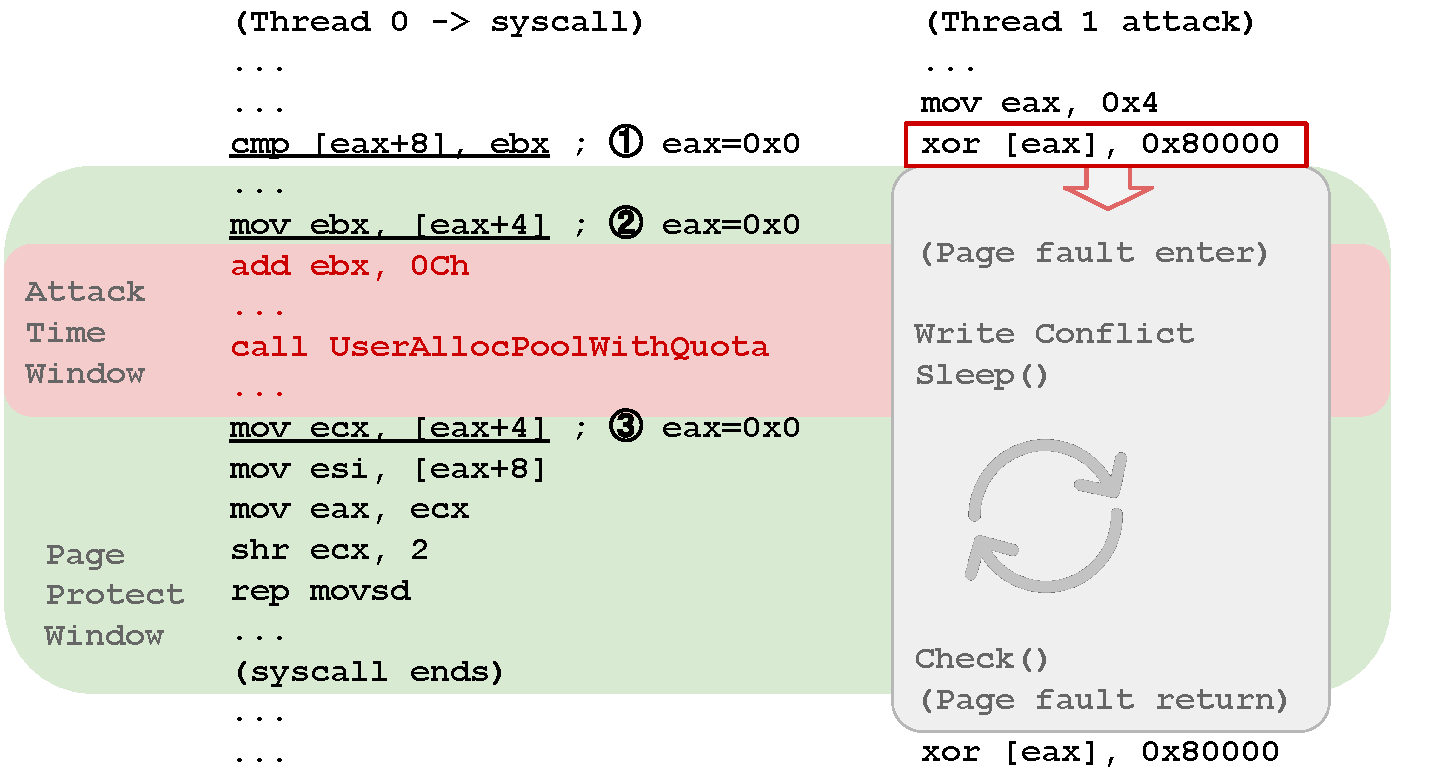
\includegraphics[width=0.47\textwidth]{figures/ms08061case2}
  \centering
  \caption{The attack thread tries to flip the data within the attack window, between instruction \texttt{\textcircled{2}} and \texttt{\textcircled{3}}. The kernel first touches the page at instruction \texttt{\textcircled{1}}, then the mitigation protects it afterward until the end of the current system call, creating the larger page-protect-window. As soon as the attack thread writes the protected page, the page fault handler suspends it until the protection ends.}
  \label{fig:ms08061case}
\end{figure}

%In the attack, as shown in ~\autoref{fig:ms08061case}, the \textcircled{2} and \texttt{\textcircled{3}} are the places where vulnerable user-mode variable pcbData are referenced, it's address is 0x4. But the first time the zero page get accessed is \textcircled{1} where several instruction ahead of \textcircled{2}, it triggers an page fault exception (cased by SMAP). Therefore this page will be marked as a kernel page by our page fault handler. From this moment until the end of the current system call, this page will be protected from modifying by either as a kernel page or a user page with read-only permit. If the attacking thread try to modified it, another page fault exception  will be raised because of access violation. Then the attacking thread will be held for 30 milliseconds before it try to re-execute the faulting instruction again, for as many as 10 times. If not possible, the attacking thread will be terminated. We can see that during the protection, memory reads at \textcircled{2} and \textcircled{3} are kept consistent.

As shown in~\autoref{fig:ms08061case}, the kernel reads the user-mode variable at address 0x4 twice at \texttt{\textcircled{2}} and \texttt{\textcircled{3}}. Any data changes during this time will cause data inconsistency in the kernel. Therefore it is the time window for the attack. The attack thread tries to enlarge the value read at \texttt{\textcircled{3}}. Our protection needs to cover the entire attack time window so that the attack thread can not change the user-mode variable during it. In this case, at \texttt{\textcircled{1}}, several instructions before \texttt{\textcircled{3}}, the CMP instruction operating on page zero, causes a SMAP exception. Our page fault handler sets page zero to kernel-mode until the current system call, that is, NtUserMessageCall(), ends. This period covers the entire attack time window. Once the attack thread tries to write the protected page, it will raise a page fault exception, and our page fault handler will suspend the current thread, waiting for the release of the page.


%\textbf{\textit{CVE-2013-1254}} is another typical TOCTOU vulnerability that found in Windows win32k module~\cite{jurczyk2013identifying}. It effects both Windows XP and Windows 7. 

%A series of same kind of vulnerability found in 26 functions of module win32k.


CVE-2013-1254. Similar to the one above mentioned, CVE-2013-1254 is another typical TOCTOU vulnerability. It is a family of 27 distinct vulnerabilities~\cite{ms13016}~\cite{jurczyk2013identifying} in the win32k module. It affects a variety of operating systems from Windows XP to Windows Server 2012.

%\begin{lstlisting}[style=code] 
%.text:BF8A993F   mov   eax, _W32UserProbeAddr
%                       .
%                       .
%.text:BF8A9973   @cmp   [ecx+8], eax@    
%.text:BF8A9976   jnb   short loc_BF8A997B
%.text:BF8A9978   @mov   eax, [ecx+8]@    
%.text:BF8A997B
%.text:BF8A997B loc_BF8A997B:                           
%.text:BF8A997B   mov   ecx, [eax]
%.text:BF8A997D   mov   eax, [eax+4]
%\end{lstlisting}
%%\captionof{lstlisting}{Flawed code in win32k.sys function SfnINOUTSTYLECHANGE()}

\begin{figure}[th]
  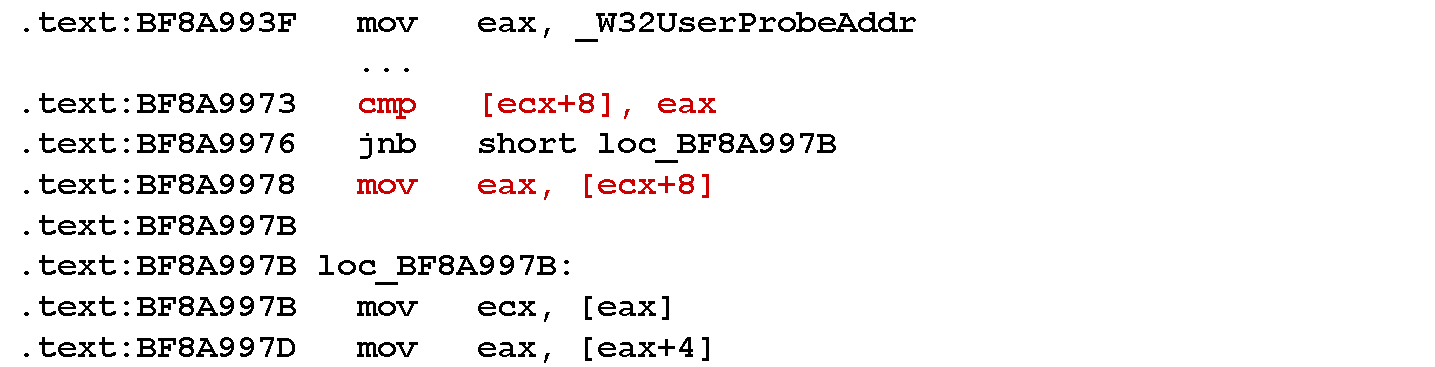
\includegraphics[width=0.47\textwidth]{figures/cve-2013-1254}
  \centering
  \caption{The family of the 27 vulnerabilities in the win32k module is mostly around the parameter sanity check. The checking code with \texttt{\_W32UserProbeAddress} makes sure that the parameters passed in reside in userspace. It is a classic time-to-check-to-time-to-use. When checking, the \texttt{[exc+8]} is less than \texttt{\_W32UserProbeAddress}, when using, it could change to a kernel address by another user-mode thread. Furthermore, the malicious address that passed the sanity check may point to an essential kernel data structure, hence gives the attacker kernel write capability.}
  \label{fig:cve-2013-1254}
\end{figure}




They have the same patterns. The code is mostly around the \texttt{\_W32UserProbeAddress}, which is a value that indicates the highest possible address for user-mode variables. As shown in~\autoref{fig:cve-2013-1254}, the flawed code in red first gets the value from \texttt{ecx+8} and compare it with \texttt{\_W32UserProbeAddress}. Afterward, it gets the data again to eax, which is the second fetch. The attacker can abuse this, changing the value to bypass the parameter sanity check, for example, send in a kernel-mode address. 


Therefore, when the instruction \texttt{cmp [ecx+8]}, eax triggers the SMAP exception, our mitigation protects this page until the current system call ends.
